
\chapter{Die Kammern der Vergessenen}
\noindent\textbf{Akt II -- Szene 4.} Offener Dungeon-Crawl bis unmittelbar vor die Statuenhalle.
\begin{meisterinfo}
\textbf{Grundprinzip:} Die Gruppe besitzt Flynns handgezeichnete Karte von 1920 und die Briefe an Helena sowie die Informationen aus M. Dyers' Buch. Die Karte bleibt gültige Grundlage der Navigation, auch wenn einige Gänge in der Wirklichkeit von der Zeichnung abweichen. Kleine leere Räume können zusammenfassend erzählt werden. Die wesentlichen Stationen -- verschüttete Kammer, Öllampe, Yusuf, Wasserstelle, Dhole, Wächterleichname und Statuenportal -- lassen sich über die Karte und die Spuren frei ansteuern. Hindernisse sind keine Einbahnstra\ss{}e; kreative Lösungen ermöglichen Alternativen. \textbf{Fortsetzung:} Die vier Statuen und das bereits geöffnete Dimensionstor erscheinen erst im folgenden Kapitel.
\end{meisterinfo}
\section{4.1 -- Der Eingang in die Tiefe}
\begin{figure}[htbp]\centering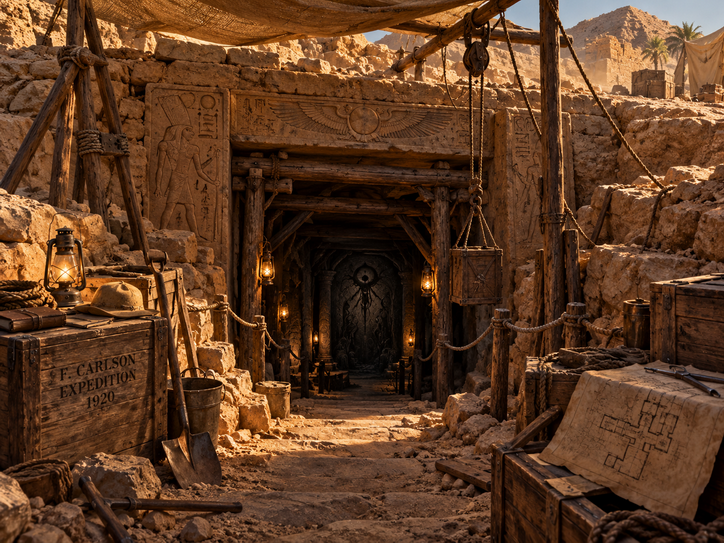
\includegraphics[width=\textwidth]{bilder/eingang-grabkammer.png}\caption{Der von der Expedition erschlossene Zugang zu den unterirdischen Kammern.}\end{figure}
\begin{vorlesetextalle}
Am Fu\ss{} einer niedrigen Felswand sichern hölzerne Stützen eine aus dem Gestein geschlagene Öffnung. Seile und eine einfache Winde hängen neben Werkzeugkisten. Eine schmale Treppe führt hinunter in das Dunkel. Mit jedem Schritt wird die Luft kühler. Das Licht Eurer Lampen tastet über Steinblöcke, verblasste Reliefs und geometrische Linien im Fels. Einige Bearbeitungsspuren sind neu, andere scheinen aus unvorstellbar ferner Zeit zu stammen. Hinter Euch schrumpft die helle Öffnung des Eingangs.
\end{vorlesetextalle}
\begin{meisterinfo}
\textbf{Archäologie:} Die Grundanlage passt nicht zu einer üblichen ägyptischen Grabanlage; manche Motive scheinen später ergänzt. \textbf{Verborgenes Erkennen:} Moderne Markierungen der Ausgräber. \textbf{Orientierung:} Bei Verwendung der Karte ist eine grundsätzliche Positionsbestimmung ohne ständigen Wurf möglich. \textbf{Horchen:} Tief unten scheint Wasser zu flie\ss{}en.
\end{meisterinfo}
\section{4.2 -- Die leeren Räume}
\begin{vorlesetextalle}
Kammer folgt auf Kammer. Manche besitzen Nischen, andere niedrige Sockel, doch alles ist leer. Auf den Böden liegt feiner Staub, in den vereinzelt die Schuhabdrücke der Expedition eingedrückt sind. Wiederholt führen breite Gänge in schmale Abzweigungen. Ihr habt das Gefühl, dass die Entfernung zwischen den Räumen auf Eurer Karte kürzer ausfällt als die Wege, die Ihr tatsächlich zurücklegt.
\end{vorlesetextalle}
\begin{meisterinfo}
\textbf{Interaktion:} Markierungen mit Kreide, Schnur oder Wegskizzen vereinfachen die Rückkehr. \textbf{Verborgenes Erkennen:} Spuren von verschobenen Steinblöcken und abgebrochene Werkzeugteile. \textbf{Archäologie:} Es fehlen typische Bestattungsmerkmale; die Anlage wirkt eher wie ein System aus Übergängen. \textbf{Keine Sackgasse:} Auch ein misslungener Orientierungswurf erzeugt Verzug, keine willkürliche Trennung der Gruppe.
\end{meisterinfo}
\section{4.3 -- Die verschüttete Kammer}
\begin{vorlesetextalle}
Ein breiter Raum ist teilweise unter einer gewaltigen Menge Sand und Geröll verschwunden. Zwischen den Massen ragen zerbrochene Stützbalken hervor; auf einem Block liegt eine Schaufel. Ein Seilende verschwindet unter dem Sand. Doch die Decke über Euch ist makellos. Nirgends zeigt sich die Bruchstelle, aus der diese Massen hätten stammen können.
\end{vorlesetextalle}
\begin{meisterinfo}
\textbf{Wiedererkennung:} Flynns Brief vom Januar berichtete von einem verschütteten Arbeiter und einer später plötzlich wieder intakten Kammer. \textbf{Geologie:} Der Sand passt mengenmä\ss{}ig nicht zum Raum. \textbf{Verborgenes Erkennen:} Ein Stück Arbeitskleidung ragt aus dem Sand. \textbf{Ausgraben:} Mit Seilen und Werkzeugen lassen sich sterbliche Überreste des Arbeiters freilegen (0/1W3 STA). Der Fund ist optional; der Raum bleibt auch ohne Freilegung bedeutend.
\end{meisterinfo}
\subsection{Die Sandfalle}
\begin{vorlesetextalle}
Ein leises Rieseln ertönt über Euren Köpfen. Zwischen den Steinplatten quillt Sand hervor. Ein dünner Strahl wird zu einer stiebenden Kaskade. Aus mehreren Wandnischen ergie\ss{}t sich trockenes Material auf den Boden. Es wird mehr -- viel mehr, als irgendwo hinter den Wänden Platz finden dürfte. Innerhalb weniger Augenblicke bedeckt Sand Eure Schuhe und steigt weiter.
\end{vorlesetextalle}
\begin{meisterinfo}
\textbf{Vier Gefahrenstufen:} (1) Knöchel, (2) Knie, (3) Hüfte, (4) Raum fast gefüllt. Nach jeder gewichtigen Handlung steigt die Stufe; clevere Hilfsmittel verzögern den Anstieg. \textbf{Lösungen:} Klettern über Nischen, Stärke zum Herausziehen, Seile als Sicherung, Mechanische Reparaturen zur Stabilisierung einer Tür, Verborgenes Erkennen für eine erhöhte Öffnung, gemeinsame Flucht über den bekannten Eingang. Misslungene Proben kosten Zeit oder Ausrüstung. Kein unvorbereiteter sofortiger Tod. \textbf{Nachwirkung:} Bei späterer Rückkehr kann der Raum vollkommen leer und unversehrt sein (1/1W4 STA). Der Widerspruch zu Flynns Briefen soll klar werden.
\end{meisterinfo}
\section{4.4 -- Dr. Skorbinsks Öllampe}
\begin{vorlesetextalle}
In einer unregelmä\ss{}igen Kammer liegen verschobene Platten und Scherben. Eine Petroleumlampe steht aufrecht mitten im Raum, als hätte jemand sie soeben dort abgestellt. Neben ihr liegen Kreide, ein beschädigtes Notizheft und ein einzelner Handschuh. Auf der Steinplatte daneben sind hastige Linien zu einem Kreis mit vier Markierungen eingeritzt.
\end{vorlesetextalle}
\begin{meisterinfo}
\textbf{Fund:} Die Lampe ist die von Flynn erwähnte Öllampe Dr. Skorbinsks. Das Heft enthält Bruchstücke: \glqq{}Der Stein reagiert nicht auf Licht. Er reagiert auf den Blick.\grqq{} / \glqq{}Die vier Wächter sind keine Abbilder. Sie bewachen etwas.\grqq{} / \glqq{}Ich glaube zu verstehen, warum die Kammern leer sind.\grqq{} \textbf{Verborgenes Erkennen:} Die vier Markierungen sind symmetrisch. \textbf{Archäologie:} Keine übliche Grabanordnung. \textbf{Okkultismus:} Vielleicht Ritual oder Mechanismus. \textbf{Mechanische Reparaturen:} Lampe reparierbar. Kein Körper des Doktors.
\end{meisterinfo}
\subsection{Der Fund des sehenden Steins}
\begin{vorlesetextalle}
Hinter einer halb verschobenen Steinplatte erkennt Ihr eine flache, sorgfältig aus dem Fels gemei\ss{}elte Nische. Darin liegt ein handtellergro\ss{}er, grauer Stein. Sein Umriss ist unregelma\ss{}ig und seine Oberfläche glatt geschliffen. Auf einer Seite befindet sich ein eigentümliches Zeichen: ein stilisiertes Auge aus einer ovalen Linie, einem Punkt und einem geschwungenen Fortsatz. Dieses Symbol kennt Ihr aus den Briefen und den Aufzeichnungen der Expedition.
\end{vorlesetextalle}
\begin{meisterinfo}
\textbf{Verbindlicher Fund:} Dies ist der \emph{sehende Stein}, das in Flynns Brief vom 5. Januar 1920 beschriebene Artefakt. Er liegt in einer Nische einer angrenzenden Kammer unweit von Skorbinsks Öllampe. Flynn berichtet am 20. Februar, den Stein erneut gefunden zu haben; nachdem er in die andere Dimension geriet, blieb er hier zurück. \textbf{Kein Wurf nötig:} Wer den Raum absucht, entdeckt die Nische und nimmt den Stein mit. \textbf{Verborgenes Erkennen:} Die umliegende Staubspur deutet auf eine erst kürzlich bewegte Platte. \textbf{Archäologie/Okkultismus:} Das Zeichen entspricht keiner eindeutig zuordenbaren ägyptischen Schrift; der Stein scheint in eine eigens dafür gearbeitete Fassung zu gehören. \textbf{Ausfallsicherung:} Wird diese Kammer ausgelassen, finden die Ermittler den Stein deutlich sichtbar unmittelbar vor dem offenen Tor in der Statuenhalle. Er ist stets zugänglich; das Finale hängt nicht von einem verdeckten Suchwurf ab. \textbf{Besitz:} Notiere, wer den Stein mitnimmt; er bleibt bis zum Einsetzen in die Plattform in dieser Person Besitz.
\end{meisterinfo}

\section{4.5 -- Die Spur von Yusuf Hassan}
\begin{vorlesetextalle}
Der Gang verengt sich an einer Kreuzung. Auf dem Boden liegt eine zerbrochene Laterne, daneben eine dunkle, eingetrocknete Spur. Jemand hat Buchstaben in die Wand gekratzt. Sie sind ungelenk und enden abrupt: \textbf{YUSUF}. Darunter findet Ihr weitere, deutlich schwächere Schriftzeichen.
\end{vorlesetextalle}
\begin{meisterinfo}
\textbf{Arabisch:} Karim el-Mady kann bei entsprechender Sprachkenntnis ohne Probe übersetzen: \glqq{}Es sieht durch uns.\grqq{} Andere Charaktere benötigen eine passende Sprachprobe oder Hilfe. \textbf{Verborgenes Erkennen:} Ein schmaler Messinganhänger mit einer eingeritzten Blüte liegt in einer Ritze. Er ähnelt dem Fund in Yusufs Tasche -- derselbe Mann erschien auf dem Atlantik. \textbf{Wahrheit für die Spielleitung:} Yusuf ist in der Anlage verschollen. Die Erscheinung an Bord war kein gewöhnlicher Geist, sondern ein räumlich-zeitliches Echo. Nicht behaupten, sein Tod sei sicher belegt; die alten Briefe berichten nur von seinem Verschwinden. \textbf{Stabilität:} Nach Erkennen der unmöglichen Verbindung optional 0/1W3.
\end{meisterinfo}
\section{4.6 -- Die unterirdische Wasserstelle}
\begin{vorlesetextalle}
Ein leises Flie\ss{}en wird zu deutlichem Rauschen. Der behauene Gang öffnet sich in eine natürliche Höhle. Feuchter Stein glänzt im Lampenlicht. Wasser sickert aus einer Felsöffnung und verschwindet unter einer niedrigen Steinbrücke. Hier unten ist die Luft überraschend kühl. In der spiegelnden Oberfläche laufen plötzlich breite Wellen auseinander, obwohl niemand das Wasser berührt hat. Von fern kommt ein tiefes, vibrierendes Grollen.
\end{vorlesetextalle}
\begin{meisterinfo}
\textbf{Geologie:} Älteres natürliches Höhlensystem; \textbf{Horchen:} Das Grollen ist nicht durch Wasser allein erklärbar. \textbf{Verborgenes Erkennen:} Breite Schleifspuren an den Wänden. \textbf{Vorbereitung:} Ein niedriger Seitenraum nahe der Wasserstelle eignet sich als Versteck. Er kann bereits vor der Dhole-Begegnung entdeckt und markiert werden.
\end{meisterinfo}
\section{4.7 -- Der Dhole}
\begin{figure}[htbp]\centering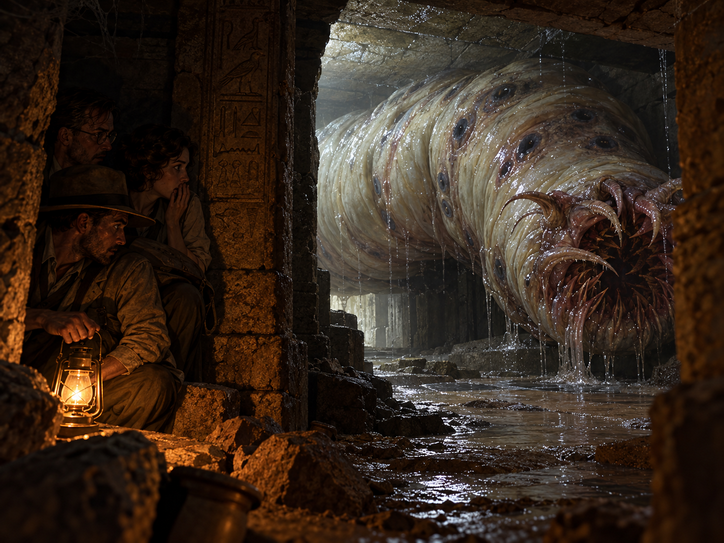
\includegraphics[width=\textwidth]{bilder/dhole.png}\caption{Der ungeheure Dhole ist eine Flucht- und Versteckbegegnung, kein gewöhnlicher Kampf.}\end{figure}
\begin{vorlesetextalle}
Ein dumpfer Schlag erschüttert den Boden, dann ein zweiter, näherer. Staub rieselt von der Decke. Ein tiefes Grollen geht in ein feuchtes, schmatzendes Schaben über. Hinter der nächsten Biegung drängt sich bleiche Masse in den Gang, viel zu gro\ss{} für jeden natürlichen Bewohner dieser Höhlen. In ihrer Oberfläche öffnen sich dunkle Vertiefungen. Vorn klafft ein ungeheures, von gebogenen Zähnen umgebenes Maul. Das Wesen schiebt sich weiter auf Euch zu und füllt fast den gesamten Gang.
\end{vorlesetextalle}
\begin{meisterinfo}
\textbf{Stabilität:} 1W4/1W10 STA (dramatischer Szenenrichtwert). \textbf{Fluchtphase:} Orientierung mit Flynns Karte zeigt einen Seitenraum; Verborgenes Erkennen entdeckt eine nahe Spalte; Klettern, Stärke und gegenseitige Hilfe bringen alle rechtzeitig in Deckung. Fehlversuche führen zu Verzögerung, verlorenen Gegenständen, leichten Verletzungen oder enger werdendem Abstand, nicht zwangsläufig sofortigem Tod. \textbf{Versteckphase:} Leise bleiben, Lampen abdecken, Schleichen oder kluge Ablenkungen einsetzen. Der Dhole verharrt vor der Öffnung, kriecht dann weiter. Ein offener Kampf ist aussichtslos. Darf durch alternative starke Idee umgangen werden.
\end{meisterinfo}
\begin{vorlesetextalle}
Ihr presst Euch in die niedrige Kammer. Kaum ist der Letzte in Sicherheit, schiebt sich das Ungeheuer unter einem tiefen Schaben am Eingang vorbei. Ein übler, feuchter Geruch dringt herein. Das Grollen bricht ab. Für einige Herzschläge bewegt sich nichts. Dann schiebt sich etwas Gewaltiges direkt vor die Öffnung. Ihr glaubt, dass es Euch wahrgenommen hat. Schlie\ss{}lich setzt das Kriechen wieder ein und entfernt sich langsam in die Tiefe.
\end{vorlesetextalle}
\subsection{Dhole -- Spielleitungswerte}
\begin{meisterinfo}
\textbf{Vereinfachter Abenteuerwert (kein regelgetreuer Abdruck):} ST 850, KO 180, GR 940, GE 15, IN 20, MA 35; TP 112, Bewegung 18 (kriechend/grabend), Panzerung 35, Verschlingen 80\%, Schleimangriff 50\%, Stabilität 1W4/1W10. \textbf{Anwendung:} Zahlen nur für unerwartete direkte Konfrontation; die Szene ist auf Ausweichen ausgelegt. Diese Werte sind vorläufig und sollten vor einer offiziellen Regelumsetzung mit der vorhandenen Dhole-Regelbuchseite abgeglichen werden.
\end{meisterinfo}
\section{4.8 -- Die Kammer der Bewahrten}
\begin{figure}[htbp]\centering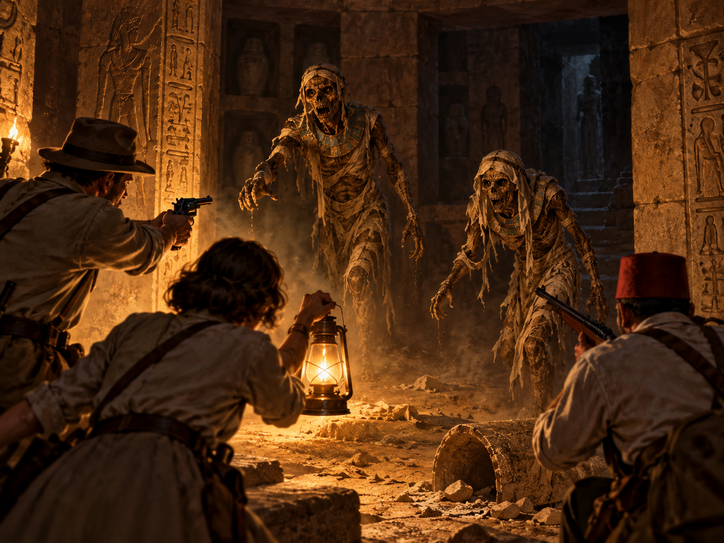
\includegraphics[width=\textwidth]{bilder/waechterleichname.png}\caption{Zwei uralte Wächterleichname schützen den Weg zur inneren Anlage.}\end{figure}
\begin{vorlesetextalle}
In einer länglichen Kammer stehen niedrige Steinsockel. Auf zweien liegen menschliche Gestalten, eingewickelt in dunkle, brüchige Leinenbinden. Harziger, trockener Geruch liegt in der Luft. Die Körper ruhen mit verschränkten Händen, den Kopf zur rückwärtigen Tür gewandt. Als Ihr Euch dieser nähert, raschelt Stoff. Eine der verdorrten Hände hebt sich.
\end{vorlesetextalle}
\begin{meisterinfo}
\textbf{Begegnung:} Zwei Wächterleichname, nicht gewöhnliche ägyptische Mumien. Sie können durch Waffen bekämpft oder umgangen werden: Engstelle nutzen, Sockel umwerfen, Ausgang blockieren, Ablenkung schaffen, Feuer an den Binden einsetzen. Keine weitere Gegnerwelle. \textbf{Stabilität:} 0/1W6 beim Anblick der sich bewegenden Toten.
\end{meisterinfo}
\subsection{Wächterleichnam -- Spielleitungswerte (je Exemplar)}
\begin{meisterinfo}
ST 70, KO 65, GR 60, GE 30, IN 10, MA 40. TP 12, Bewegung 5, Panzerung 2 (verhärtete Haut und Binden), Klauen 40\%, Schaden 1W4 + 1W4 Schadensbonus, Ausweichen 15\%, Stabilität 0/1W6. Die Wächter sind langsame, eigens für diese Szene entworfene Gegner. Sie reagieren auf Erschütterungen und den Durchgang zur inneren Kammer. \textbf{Belohnung für Planen:} Wer Nischen, Türrahmen, Seile oder mitgebrachte Geräte nutzt, kann einen Kampf vermeiden oder abkürzen.
\end{meisterinfo}
\section{4.9 -- Vor dem Portal der vier Wächter}
\begin{vorlesetextalle}
Ein breiter Gang führt tiefer in den Fels. Seine Wände sind ungewöhnlich glatt, die Bodenplatten dunkel und präzise gefügt. Geometrische Zeichen wiederholen sich entlang des Weges, manche ähneln dem Symbol auf dem sehenden Stein. Dann öffnet sich der Gang zu einem Vorraum. Vier niedrige Säulen stehen symmetrisch an den Wänden. Dahinter erhebt sich der breite, mit dunklen Zeichen versehene Durchgang zur eigentlichen Statuenhalle. Durch ihn dringt ein ungewöhnlich kalter Luftzug. Jenseits liegt ein gro\ss{}er Raum in tiefem Schatten; weiter hinten zeichnet sich ein gigantisches steinernes Tor ab. Zu Eurer Verwunderung ist der Boden auf dem Weg dorthin vollkommen frei von Staub.
\end{vorlesetextalle}
\begin{meisterinfo}
\textbf{Archäologie:} Vier symmetrische Säulen als Teil einer Konstruktion. \textbf{Verborgenes Erkennen:} Spuren eines älteren gewaltsamen Öffnungsversuchs. \textbf{Okkultismus:} Vier Positionen umschlie\ss{}en möglicherweise ein Zentrum. \textbf{Karte:} Die Gruppe steht vor dem von Flynn markierten Bereich der vier Statuen. \textbf{Szenenende:} Noch keine Lösung für die Statuen oder das Dimensionstor festlegen; das ist Gegenstand der nächsten Szene. Ermögliche Rückkehr, Rast und letzte Ausrüstungschecks.
\end{meisterinfo}
